\documentclass[a4paper, 12pt]{article}

%%%%%%%%%%%%%%%%%%%%%%%%%%%%%%% PACKAGES %%%%%%%%%%%%%%%%%%%%%%%%%%%%%%%
% Math-related things
\usepackage{amsmath}
\usepackage{amssymb}
\usepackage{amsthm}
% Italian spelling
\usepackage[italian]{babel}
% Accenti e caratteri speciali
\usepackage[utf8]{inputenc}
% Margini e grafica della pagina
\usepackage[top=2cm, bottom=2cm, left=2cm, right=2cm]{geometry}
\usepackage{fancyhdr}
% Tabelle
\usepackage{tabularx}
% Graphs and Images handling
\usepackage{graphicx}
\usepackage{svg}
% VHDL language support
\usepackage{minted}
% Hypertext references
\usepackage{hyperref}
% Citations
\usepackage{epigraph}

% Title Page
\title{Eriantys - Prova Finale di Ingegneria del Software}
\author{
	Paolo Pertino [10729600]
	\href{mailto:paolo.pertino@mail.polimi.it}{paolo.pertino@mail.polimi.it} \\
	Leonardo Pesce [10659489]
	\href{mailto:leonardo.pesce@mail.polimi.it}{leonardo.pesce@mail.polimi.it} \\
	Alberto Paddeu [10729194]
	\href{mailto:alberto.paddeu@mail.polimi.it}{alberto.paddeu@mail.polimi.it} \\
} 

% Contents page settings
\renewcommand*\contentsname{Indice}
\setcounter{tocdepth}{3}

\newcommand{\quantities}[1]{%
	\begin{tabular}{@{}c@{}}\strut#1\strut\end{tabular}%
}

% General page settings
\pagestyle{fancy}
\fancyhf{}
\rhead{\leftmark}
\lhead{Eriantys - Prova Finale di Ingegneria del Software}
\cfoot{\thepage}

% Hyperrefs setup
\hypersetup{
	colorlinks=true,
	linkcolor=[rgb]{0.996,0.396,0.090196}, %254 101 23
	filecolor=magenta,      
	urlcolor=[rgb]{0.72156862745,0.0078431372549,0.00392156862745},
	citecolor=[rgb]{0.517647,0.0156862745,0.0117647},
	pdftitle={Eriantys - Prova Finale di Ingegneria del Software},
	pdfpagemode=FullScreen,
}

\begin{document}
	\pagenumbering{gobble}
	\date{\today}
	\maketitle
	\newpage
	\pagenumbering{arabic}
	
	\tableofcontents
	
	\newpage
	\section{Introduzione}
	\paragraph{}
	La \textbf{Prova Finale di Ingegneria del Software} dell'anno scolastico 2021-2022 prevede lo sviluppo di una versione software del gioco da tavolo \emph{Eriantys}, un prodotto \emph{Cranio Creations}\cite{eriantys} che si ispira e tenta di rinnovare il già affermato \emph{Carolus Magnus}\cite{carolusMagnus}.
	
	\paragraph{}
	Il prodotto finale dovrà soddisfare i requisiti \emph{Game-Specific} e \emph{Game-Agnostic} indicati nel documento \emph{requirements.pdf}. In particolare è richiesto l'utilizzo del design pattern \emph{Model-View-Controller} di cui a breve forniremo una concisa descrizione.\\
	Per incrementare il punteggio ottenuto, il team si concentrerà nell'implementazione delle regole complete del gioco, nel fornire la possibilità ai giocatori di connettersi al server e giocare tramite un'interfaccia a linea di comando (CLI) oppure mediante l'interazione con un'interfaccia grafica (GUI). Infine si darà spazio all'implementazione di quante più possibili delle seguente funzionalità aggiuntive: \emph{12 carte personaggio, partite a 4 giocatori, partite multiple e persistenza}.
	
	\subsection{Model-View-Controller}
	\paragraph{}
	Il \emph{Model-View-Controller} è un design pattern per la progettazione di un'architettura software. Esso permette di separare la logica di presentazione dell'applicativo da quella applicativa(o detta di business).\\
	\begin{figure}[h!]
		\centering
		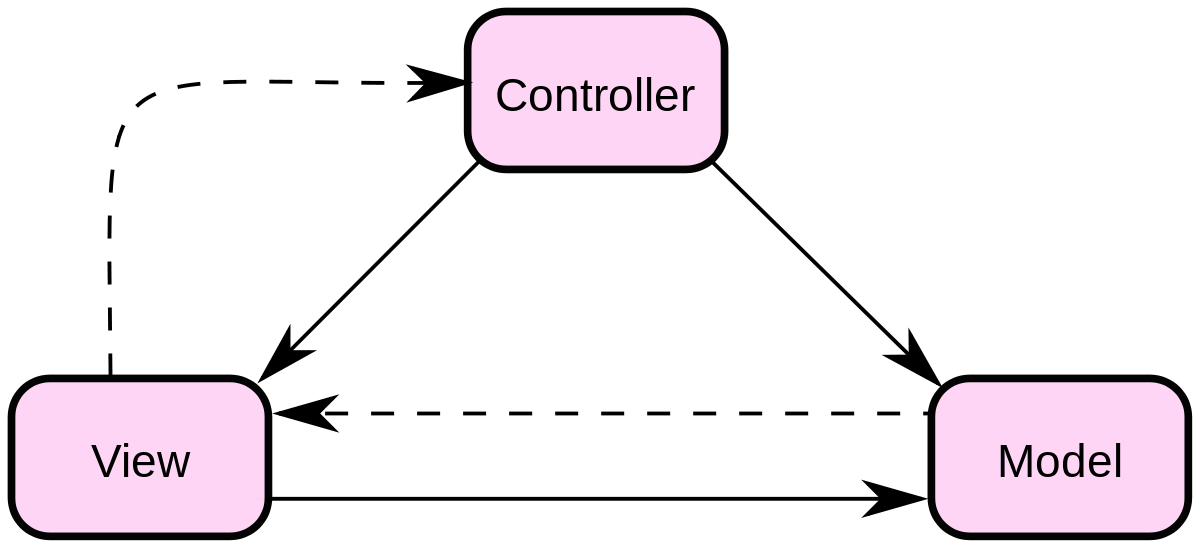
\includegraphics[scale=0.35]{mvc.png}
		\caption{Model-View-Controller Pattern}
	\end{figure}
	
	Come deducibile dal nome, tale architettura è strutturata su 3 differenti layer:\\
	\begin{enumerate}
		\item \emph{Model} - gestione diretta dei dati, della logica e delle regole del programma. Si noti come l'utente non modifica in modo diretto lo stato del model, bensì si interfaccia con il controller il quale gestisce in separata sede l'interazione con lo stato interno del sistema;
		\item \emph{View} - permette la visualizzazione dello stato del model e gestisce l'interazione con gli utenti e agenti esterni; 
		\item \emph{Controller} - riceve i comandi dell'utente attraverso la view e li attua modificando gli stati degli altri due layers.
	\end{enumerate}
	Sono possibili viste multiple di uno stesso modello. Nel nostro caso, infatti, saranno implementate due viste: il gioco sarà pertanto accessibile sia attraverso linea di comando sia mediante interfaccia grafica.
	
	\newpage
	\section{Devlog}
	\paragraph{}
	Nella seguente sezione riportiamo settimana per settimana i progressi effettuati dal team, evidenziando, ove necessario, eventuali diagrammi e gli snodi del ragionamento.
	\subsection{Settimana 1: Un primo sguardo al class diagram del Modello}
	\paragraph{}
	Durante la prima settimana di corso abbiamo analizzato i componenti fisici del gioco e le sue regole, cercando di riprodurre uno schema logico di tali elementi attraverso un \emph{Class Diagram UML}. Esso contiene una prima bozza della struttura del Model:\\
	\begin{figure}[h]
		\centering
		\def\svgwidth{\columnwidth}
		\resizebox{\linewidth}{!}{\input{umlFirstWeek.pdf_tex}}
		\caption{Class Diagram del Model - Bozza}
	\end{figure}\\
	Come indicato, lo schema sopra riportato è una bozza primitiva e di seguito riportiamo i principali ragionamenti effettuati:\\
	\begin{itemize}
		\setlength{\parskip}{0pt}
		\setlength{\parsep}{0pt}
		
		\item Tutti i componenti fisici, in futuro, avranno una loro grafica che dovrà essere mostrata. Pertanto implementano l'interfaccia GameObject che prevede l'implementazione di un metodo specifico per conseguire tale obiettivo.
		\item Il cerchio di isole che costituisce la board di gioco è stato pensato come \emph{Doubly Circular Linked List}\cite{circularDoublyLinkedList}. Con tale rappresentazione sarà più agevole lo spostamento di madre natura e l'operazione di merge di 2 isole consecutive a valle della loro conquista da parte di un giocatore.
		\item Volendo implementare le regole complete, quindi prevedendo la possibilità di giocare una partita seguendo la modalità per esperti, e tenendo conto della possibilità di implementare partite multiple sullo stesso server, ci siamo interrogati su come far impattare tale scelta sui diversi metodi delle varie classi. L'idea è quindi quella di utilizzare un Template Pattern creando una classe astratta di gioco dalla quale saranno derivate le 3 versioni di gioco (per 2, 3 e 4 giocatori). Da esse discenderanno successivamente le corrispettive versioni a 2, 3 e 4 giocatori in modalità per esperti.
		\item In vista dell'implementazione della funzionalità di persistenza della partita, è stato brevemente analizzato il pattern \emph{Memento} ed il suo funzionamento per capire se esso possa essere utile in futuro.
	\end{itemize}
	\subsection{Settimana 2: Eriantys Model}
	\paragraph{}
	Nella seconda settimana è stato scritto parte del codice del model, identificando i punti critici in cui è richiesta un'interazione con l'utente. Inoltre è stata rifinita la struttura del model che riportiamo di seguito aggiornata:\\
	\begin{figure}[h]
		\centering
		\def\svgwidth{\columnwidth}
		\resizebox{\linewidth}{!}{\input{umlSecondWeek.pdf_tex}}
		\caption{Class Diagram del Model - Seconda settimana}
	\end{figure}\\
	É stata prestata attenzione a:
		\begin{itemize}
		\setlength{\parskip}{0pt}
		\setlength{\parsep}{0pt}
		
		\item individuare un flow di operazioni che contraddistinguono la partita (una volta connessi i giocatori, finchè non è presente un vincitore vengono eseguite Planning Phase, Action Phase rispettivamente per tutti i giocatori continuamente)
		\item studiare il meccanismo delle carte personaggio per l'implementazione della modalità per esperti più approfonditamente
		\item restyle del diagramma UML per renderlo coerente con il codice scritto
	\end{itemize}

	% Week 3: Model update & Controller
	\newpage
	\subsection{Settimana 3: Eriantys Model update e Controller}
	\paragraph{}
	Nella terza settimana è stato rivisitato e riscritto parte del codice del model e implementato la parte di controller. Tra le varie modifiche le più importanti risultano essere la nuova implementazione della classe Game che adesso risulta essere accorpata nelle varie versioni da 2, 3 e 4 giocatori, la nuova versione per l'implementazione delle carte avanzate e il ribilanciamento del carico tra controller e la classe game. \\
	\begin{figure}[h]
		\centering
		\def\svgwidth{\columnwidth}
		\resizebox{\linewidth}{!}{\input{{umlThirdWeek.pdf_tex}}}
		\caption{Class Diagram - Terza settimana}
	\end{figure}\\
	Seguendo l'ordine sopra elencato delle modifiche:
	\begin{itemize}
		\setlength{\parskip}{0pt}
		\setlength{\parsep}{0pt}
		
		\item \textbf{Modifica struttura del game:} Visto che dalle precedenti implementazioni le modifiche effettive nelle istanze di gioco a 2, 3 e 4 giocatori erano poche, è stato ripensato un modo per unirle trasformando la classe game in una generica che varia gli effetti dei suoi metodi in base al numero di giocatori assegnati inizialmente. Ciò non ha implicato alcun uso di \emph{if} o \emph{switch} aggiuntivi in quanto con opportuni accorgimenti e con l'uso della funzione modulo $\%$ si sono potute trasformare le funzioni da specifiche a generiche in modo trasparente rispetto il numero di giocatori. 
		Questa unione ha comportato anche il collasso delle tre precedenti classi avanzate, che a livello pratico implementavano lo stesso codice, in una unica.
		Tutto ciò a portato ad avere un codice più snello e pulito senza eccessive ripetizioni.
		\item \textbf{Nuove carte avanzate:} Per implementare più carte personaggio possibili cercando di rendere trasparente l'aggiunta delle stesse alle meccaniche di base del gioco, è stato ripensato come esse vengono implementate. Adesso l'attivazione del loro effetto è circoscritta nel metodo \emph{playEffect} della classe rappresentante la carta stessa. A seguito dell'attivazione con successo di una delle suddette carte, la funzione playEffect provvederà a manipolare l'istanza della classe \emph{game} settando temporaneamente dei calcolatori particolari (vedi calcolatore di influenza e update dell'ownership del professore) oppure modificando di fatto lo stato di alcuni componenti del game stesso. Tali modifiche saranno opportunamente gestite, se necessario, alla fine del turno del giocatore che ha attivato la carta. 
		\item \textbf{Ribilanciamento tra Model e Controller:} abbiamo notato che molti metodi appartenenti alla classe controller erano stati implementati inizialmente nel model, questi sono stati spostati e verificati in modo da ribilanciare il peso tra i due componenti.
	\end{itemize}
	
	% Peer Review subsubsection to describe briefly our model
	\subsubsection{Peer Review - UML}
	\paragraph{}
	In vista dell'attività di \textbf{peer review} prevista per la \emph{quarta} settimana di lavoro, forniamo una breve descrizione di alcuni componenti della nostra struttura del modello che riteniamo importanti:\\
	\begin{figure}[h!]
		\centering
		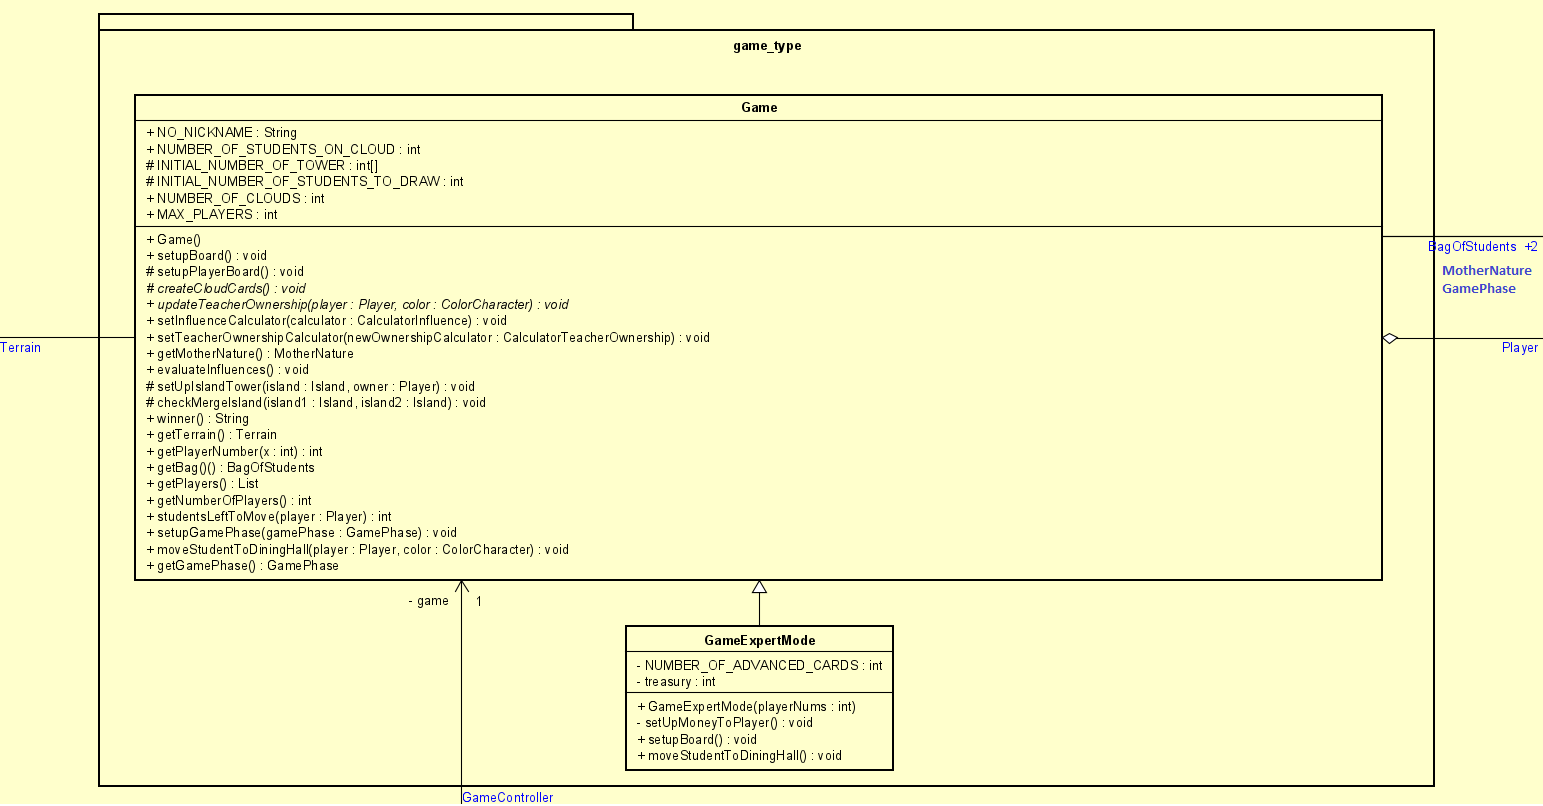
\includegraphics[scale=0.50]{game class.png}
		\caption{Game Class}
	\end{figure}\\
	\paragraph{}
	La classe Game è il fulcro della nostra struttura. Riassumiamo infatti in tale oggetto tutti i componenti del gioco, quali gli oggetti che compongono il terreno (isole, carte nuvola), i giocatori (players), madre natura, il sacchetto di studenti e i calcolatori di influenza e condizioni di possesso dei professori. Il controller si interfaccerà inizialmente con questa classe per accedere agli oggetti del modello da modificare.\\
	Dalla Game class, si dirama GameExpertMode ovvero il gioco in modalità per esperti. Quest'ultima non modifica in modo netto le funzionalità di base del gioco, ma in certi casi le arricchisce. Pertanto, è stato fatto l'override dei metodi che modificano, seppur parzialmente, il comportamento da assumere in talune situazioni.
	\newpage
	\begin{figure}[h!]
		\centering
		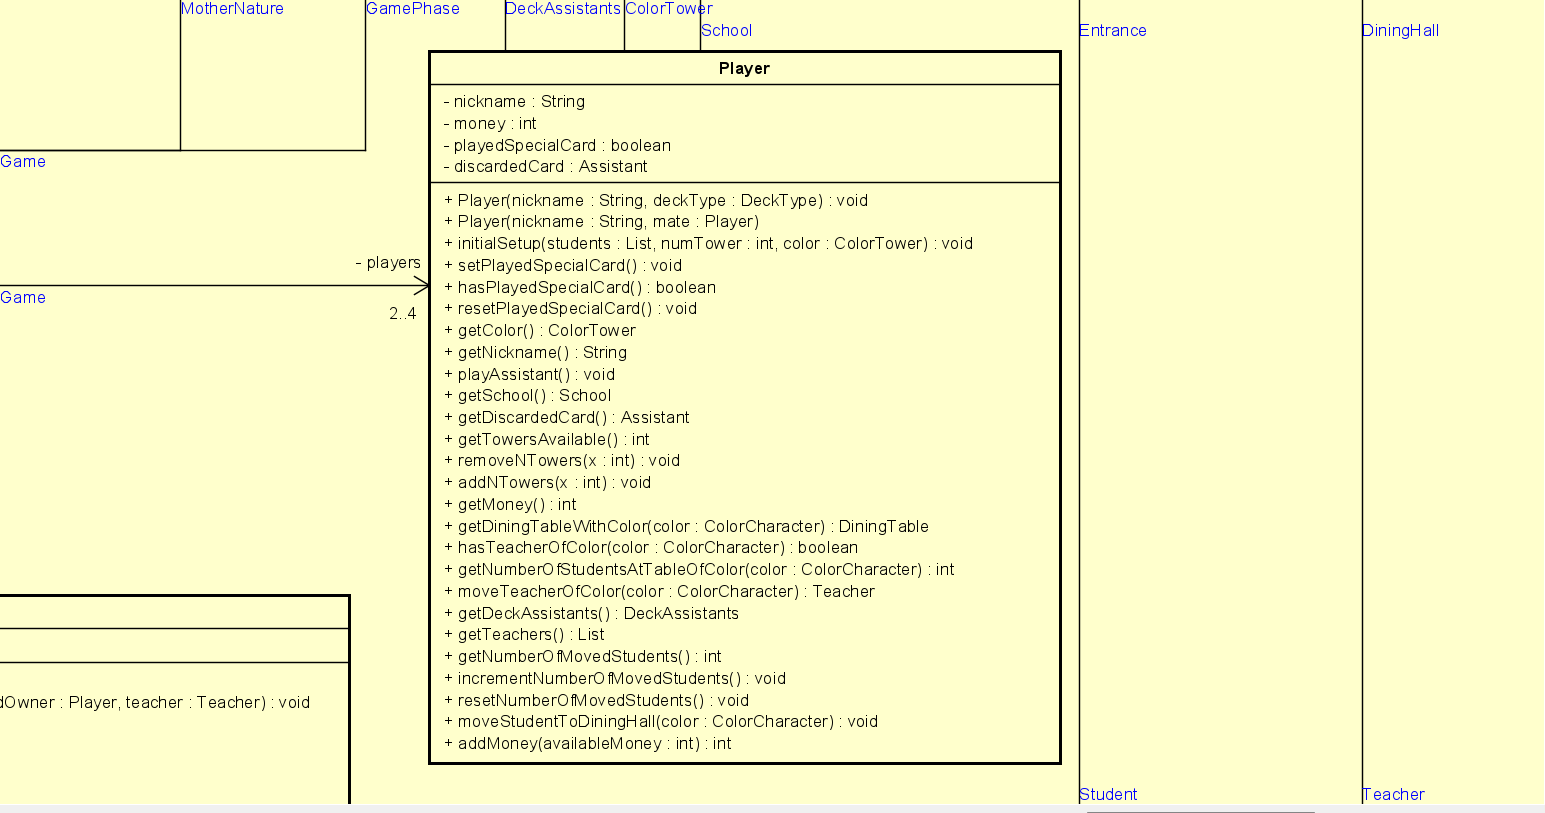
\includegraphics[scale=0.5]{player class.png}
		\caption{Player Class}
	\end{figure}
	\paragraph{}
	La classe player riassume tutte le proprietà di un giocatore, dal suo nickname, al suo mazzo di carte assistente, alla sua plancia di gioco...\\
	Ogni giocatore avrà quindi una corrispettiva rappresentazione all'interno del modello che ne conterrà lo stato per tutto il corso della partita.\\
	\begin{figure}[h!]
		\centering
		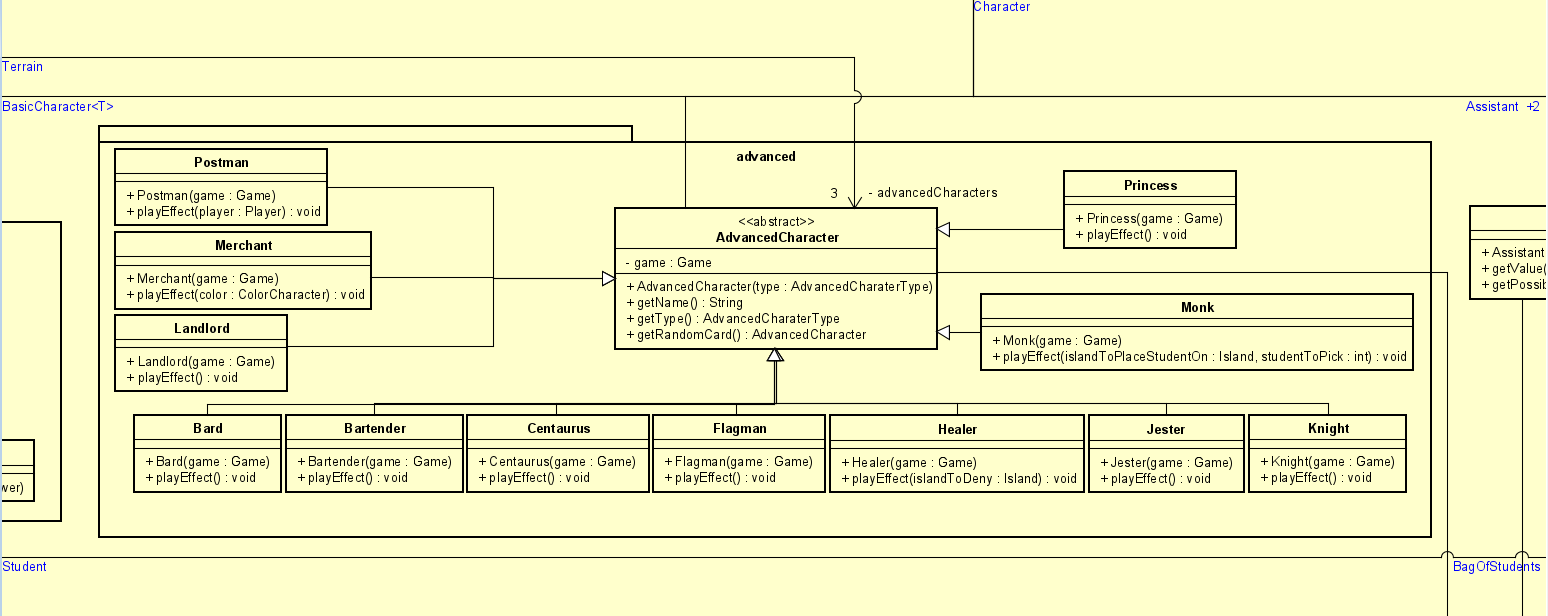
\includegraphics[scale=0.5]{advanced class.png}
		\caption{AdvancedCharacter Class \& Implementazione Personaggi}
	\end{figure}
	\paragraph{}
	La sezione \emph{advanced} contiene le carte personaggio. Come detto in precedenza, per rendere trasparente ed estendibile l'implementazione delle suddette carte, abbiamo deciso di utilizzare una classe per ciascun personaggio. Comune a tutti è la presenza di un riferimento al game in modo tale che il metodo playEffect possa decorare, a seconda della carta, la funzionalità di interesse seguendo la specifica.
	
	\newpage
	\begin{figure}[h!]
		\centering
		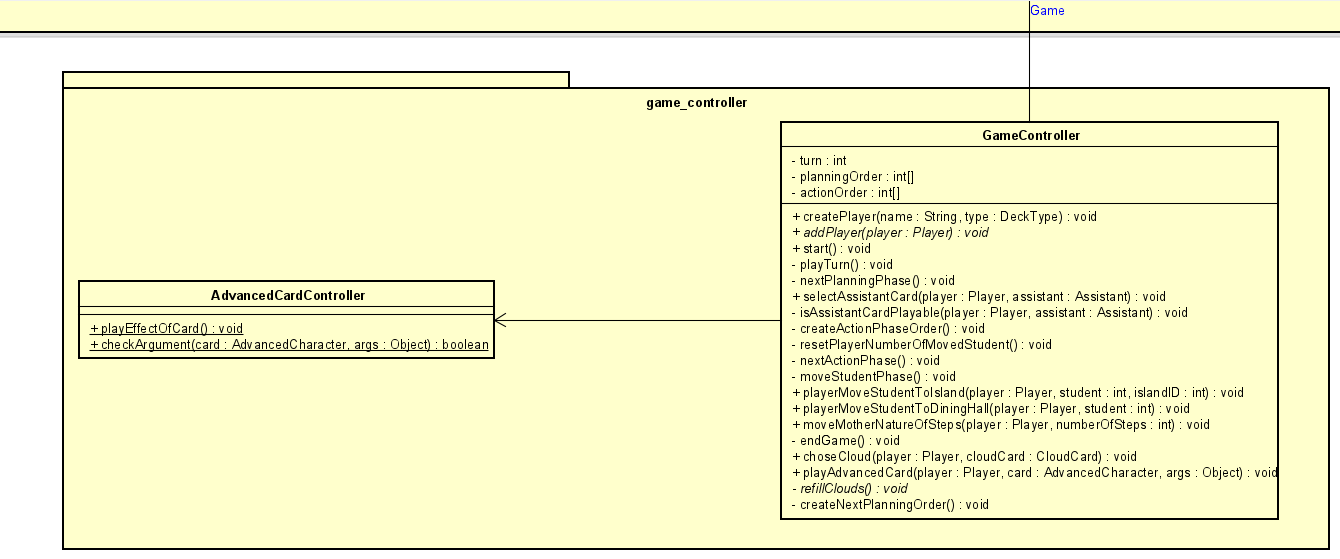
\includegraphics[scale=0.5]{controller.png}
		\caption{Controller}
	\end{figure}
	\paragraph{}
	Riportiamo infine per completezza una breve descrizione dell'idea che ci siamo fatti del controller. Di seguito forniamo una breve descrizione dei metodi principali che \emph{dovrebbero} riassumere i possibili comandi che un giocatore deve poter eseguire (ogni metodo è responsabile di effettuare i controlli sulla fattibilità della mossa richiesta):
	\begin{itemize}
		\item \emph{createPlayer \& addPlayer} rispondono alla volontà del giocatore di iscriversi alla partita in fase di creazione con i parametri indicati;
		\item \emph{start} fa iniziare il match;
		\item \emph{selectAssistantCard} fa giocare al giocatore la carta assistente da lui selezionata;
		\item \emph{playerMoveStudentToIsland} permette al giocatore di muovere lo studente selezionato dal suo ingresso all'isola selezionata;
		\item \emph{playerMoveStudentToDiningHall} permette al giocatore di muovere lo studente selezionato dal suo ingresso alla sua sala;
		\item \emph{moveMotherNatureOfSteps} permette al giocatore di muovere madre natura della quantità di passi indicata (valutazione dell'influenza delle isole, eventuale costruzione di torri e merge di isolotti adiacenti sono operazioni interne triggerate a fine del movimento di madre natura);
		\item \emph{choseCloud} permette al giocatore di prelevare gli studenti dalla cloud card selezionata;
		\item \emph{playAdvancedCard} permette al giocatore di giocare l'effetto della carta personaggio selezionata.
	\end{itemize}
	
	% Week 4: Teting del modello
	\newpage
	\subsection{Settimana 4: Testing del Modello}
	\paragraph{}
	Nella quarta settimana di sviluppo è stata consolidata la struttura del nostro modello analizzando nuovamente l'implementazione delle carte avanzate. Sono inoltre stati testati buona parte dei metodi del Model, come quelli inerenti al calcolo dell'influenza su un'isola, verifica delle condizioni di ownership dei professori, merging di isole adiacenti conquistate da uno stesso giocatore, etc...\\
	Riportiamo di seguito, per completezza, la versione del diagramma UML aggiornata alla quarta settimana:\\
	\begin{figure}[h]
		\centering
		\def\svgwidth{\columnwidth}
		\resizebox{\linewidth}{!}{\input{{umlFourthWeek.pdf_tex}}}
		\caption{Class Diagram - Quarta settimana}
	\end{figure}\\
	
	\paragraph{}
	Infine è stato stilato il documento di Peer-Review del gruppo GC13 (vedi \emph{/Deliverables/Peer Reviews/Peer-Review-1-UML-GC13.pdf}).
	
	% Week 5: controller tests & network arch init
	\newpage
	\subsection{Settimana 5: Controller tests ed architettura di rete}
	\paragraph{}
	Nella quinta settimana di sviluppo sono stati testati i metodi del controller per verificarne il comportamento atteso a valle di test cases standard. Inoltre, in vista dell'introduzione della rete, il controller è stato corredato da diversi oggetti rappresentanti le azioni e richieste che il giocatore vuole eseguire durante una partita.\\
	\begin{figure}[h!]
		\centering
		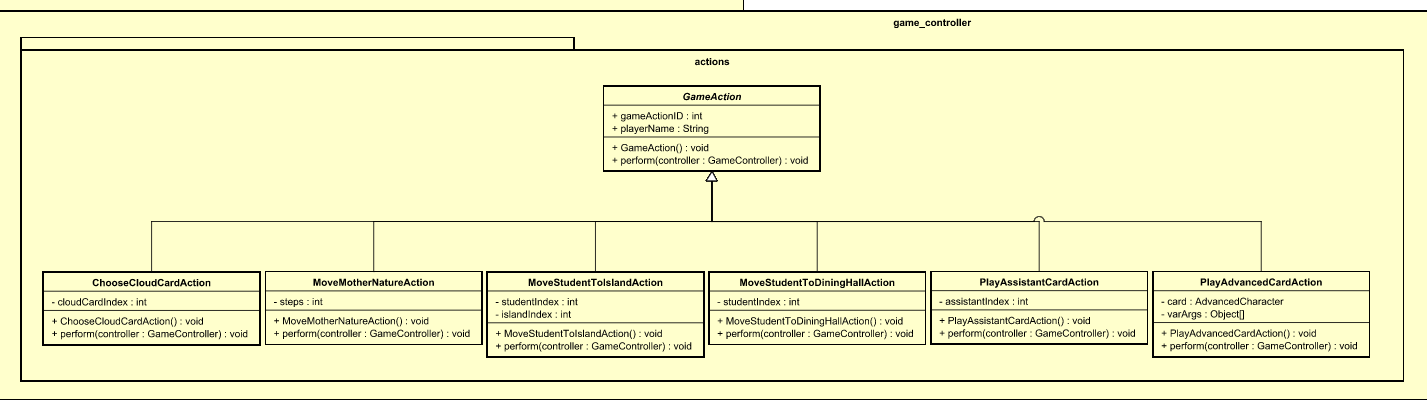
\includegraphics[scale=0.55]{gameActions.png}
		\caption{Controller game actions}
	\end{figure}
	\paragraph{}
	Tali azioni saranno oggetto di scambio tra client e server per gestire l'applicazione di azioni da parte del controller sul modello. Il metodo \textit{perform} di ogni azione, infatti, esegue l'operazione chiamando i rispettivi metodi del controllore con i dovuti parametri.\\
	Infine, a seguito dell'esercitazione svolta su \emph{Socket e Serializzazione} è stata inserita una prima versione dell'architettura di rete.
	
	% Week 6: Network & CLI initialization
	\subsection{Settimana 6: Network multi-partita e CLI}
	\paragraph{}
	Nel corso della sesta settimana di sviluppo abbiamo parallelamente aggiornato la nostra struttura di rete ed implementato un'iniziale versione di interfaccia utente da linea di comando.\\
	\begin{figure}[h]
		\centering
		\def\svgwidth{\columnwidth}
		\resizebox{\linewidth}{!}{\input{{umlFifth&SixthWeek.pdf_tex}}}
		\caption{Class Diagram - Quinta e Sesta settimana}
	\end{figure}
	\paragraph{}
	Siamo pertanto riusciti a testare la nostra implementazione fino a poter giocare una partita completa con le regole standard. Di seguito riportiamo un elenco delle attività svolte:\\
	\begin{itemize}
		\item Interfaccia grafica da linea di comando. Fa uso di codici di escape ANSI per gestire i colori.
		\item Implementazione della funzionalità avanzata "Partite Multiple" attraverso un sistema di gestione a Lobby.
		\item Macchina a stati (?)
		\item Gestione disconnessioni (?)
		\item Messaggi scambiati (?)
	\end{itemize}


	% Strumenti usati
	\newpage
	\section{Strumenti utilizzati}
	Nella seguente sezione verranno indicati i principali strumenti di sviluppo utilizzati:\\
	\begin{itemize}
		\setlength{\parskip}{0pt}
		\setlength{\parsep}{0pt}
		
		\item \emph{IntelliJ IDEA Ultimate 2021.3.2} - Principale IDE utilizzato.
		\item \emph{Maven} - Gestione dello sviluppo del progetto software e di tutte le sue fasi.
		\item \emph{JUnit} - Framework principale di unit testing.
		\item \emph{AstahUML} - Creazione di diagrammi UML.
		\item \emph{GitKraken} - Git GUI per visualizzare il workflow di sviluppo ed utilizzare efficientemente Git.
		\item \emph{TEXStudio} - Gestione e aggiornamento del report.
	\end{itemize}
	% Bibliografia
	\newpage
	\begin{thebibliography}{99}
		\bibitem{eriantys}
		\href{https://www.craniocreations.it/prodotto/eriantys/}{Eriantys, Cranio Creations}
		
		\bibitem{carolusMagnus}
		\href{https://www.goblins.net/giochi/carolus-magnus-5071}{Carolvs Magnvs, Winning Moves}
		
		\bibitem{circularDoublyLinkedList}
		\href{https://www.softwaretestinghelp.com/doubly-linked-list-in-java/#Circular_Doubly_Linked_List_In_Java}{Circular Doubly Linked List}
		
	\end{thebibliography} 
\end{document}         
